\documentclass{article}

\usepackage[utf8]{inputenc}
\usepackage[backend=biber, style=ieee]{biblatex}
\usepackage[a4paper, total={170mm,257mm}, left=20mm, top=20mm]{geometry}
\usepackage{graphicx}
\usepackage{titling}
\usepackage{amsfonts}
\usepackage{amsmath}
\usepackage{lmodern}
\usepackage{physics}
\usepackage{tikz}
\usepackage{pgfplots}
\usepackage{fancyvrb}
\usepackage{pmboxdraw}
\usepackage{fancyhdr}

\pgfplotsset{compat=1.18}
\usetikzlibrary{calc}
\setlength{\headheight}{5mm}

\addbibresource{citations.bib} %Imports bibliography file
 
\fancypagestyle{plain}{%  the preset of fancyhdr 
  \fancyhf{} % clear all header and footer fields
  \fancyhead[L]{UML Project Proposal}
  \fancyhead[R]{\theauthor}
}

\makeatletter
\def\@maketitle{%
  \newpage
  \null
  \vskip 1em%
  \begin{center}%
  \let \footnote \thanks
    {\LARGE \@title \par}%
    \vskip 1em%
    %{\large \@date}%
  \end{center}%
  \par
  \vskip 1em}
\makeatother

\title{Computing Hierarchical Embeddings of File Contents Using File System Tree Distance Metrics}
\author{Alex Chen, Gilbert Yang, Geoffrey Wu}

\begin{document}

\maketitle

% \section{Introduction}

% \cite{sarkar2011low}
% \cite{sala2018representation}
% \cite{murtagh2012algorithms}
% \cite{paszke2019pytorch}
% \cite{llama3modelcard}
% \cite{celinska2024numerical}

% \begin{align}
%   \min_{f} \sum_{(u_i,u_j) \in U^2} \Big[ \rho(f(\phi(u_i)),f(\phi(u_j)) - T(u_i,u_j) \Big]^2 \;  \label{eq:objective}
% \end{align}

\section{Introduction}

\subsection{Related Work}

% TODO: literature review
[Literature review]

\section{Background}

We present a brief overview of concepts that are used in our project.

\subsection{Metric Spaces and Embeddings}

A metric space is a set $X$ equipped with a distance function $\rho: X \times X \rightarrow \mathbb{R}$ that gives the distance between pairs of elements. $\rho$ must satisfy the following properties for all $x,y,z \in X$:

\begin{enumerate}
  \item Non-negativity: $\rho(x,y) \geq 0$.
  \item Positivity: $\rho(x,y) = 0$ if and only if $x = y$.
  \item Symmetry: $\rho(x,y) = \rho(y,x)$.
  \item Triangle inequality: $\rho(x,y) \leq \rho(x,z) + \rho(z,y)$.
\end{enumerate}

\subsubsection{Trees as Metric Spaces}

Consider a set $X$ where elements are nodes in a tree. A valid distance function $\rho$ can be defined as the length of the shortest path between two nodes. This satisfies the properties of a metric space.

\begin{figure}[ht]
  \centering
  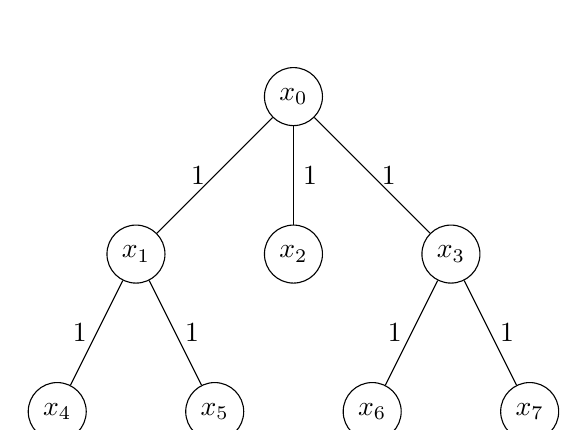
\begin{tikzpicture}
    % Nodes
    \node[circle, draw] (A) at (0,0) {$x_0$};
    \node[circle, draw] (B) at (-2,-2) {$x_1$};
    \node[circle, draw] (C) at (0,-2) {$x_2$};
    \node[circle, draw] (D) at (2,-2) {$x_3$};
    \node[circle, draw] (E) at (-3,-4) {$x_4$};
    \node[circle, draw] (F) at (-1,-4) {$x_5$};
    \node[circle, draw] (G) at (1,-4) {$x_6$};
    \node[circle, draw] (H) at (3,-4) {$x_7$};

    % Edges with distances
    \draw (A) -- node[midway, fill=none, left] {$1$} (B);
    \draw (A) -- node[midway, fill=none, right] {$1$} (C);
    \draw (A) -- node[midway, fill=none, right] {$1$} (D);
    \draw (B) -- node[midway, fill=none, left] {$1$} (E);
    \draw (B) -- node[midway, fill=none, right] {$1$} (F);
    \draw (D) -- node[midway, fill=none, left] {$1$} (G);
    \draw (D) -- node[midway, fill=none, right] {$1$} (H);
  \end{tikzpicture}
  \caption{An illustration of a tree metric space. In general, edge lengths are not necessarily equal. As an example, the distance between $x_2$ and $x_4$ is $3$.}
  \label{fig:tree-metric-space}
\end{figure}

\subsubsection{Distance-Preserving Embeddings}

Given elements of a metric space, we are often interested in embedding them into a lower-dimensional space in a way that preserves distances. Formally, an embedding is a mapping $f: X \rightarrow Y$, from metric space $(\rho, X)$ to metric space $(\sigma, Y)$. To preserve distances means to find an $f$ such that for all $x,y \in X$, $\sigma(f(x),f(y)) \approx \rho(x,y)$. Later, we will discuss ways of quantifying the quality of an embedding.

\subsection{Hyperbolic Geometry}

Hyperbolic geometry is a non-Euclidean geometry characterized by a constant negative curvature. Hyperbolic spaces are natural candidates for embedding trees \cite{sarkar2011low}. Many models of hyperbolic space exist, including the hyperboloid, Poincaré disk, Poincaré half-plane, and Klein disk models. We will focus on the Poincaré disk model because it is easy to visualize.

\subsubsection{Poincaré Disk Model}

The Poincaré disk model of hyperbolic space maps points in the hyperbolic plane to points in the unit disk (in Euclidean space). The distance between two points with coordinates $\mathbf x_1$ and $\mathbf x_2$ in the \emph{ambient} Euclidean space is
\begin{align}
  d(\mathbf x_1, \mathbf x_2)
  = \text{arcosh} \qty[1 + 2 \frac{\norm{\mathbf x_1 - \mathbf x_2}^2}{\qty(1 - \norm{\mathbf x_1}^2) \qty(1 - \norm{\mathbf x_2}^2)}] \; . \label{eq:poincare-distance}
\end{align}

Geodesics are defined as the shortest paths between two points. In the Poincaré disk model, geodesics are arcs of circles that intersect the boundary of the disk at right angles. For any two points in the Poincaré disk, there is a unique geodesic connecting them.

\begin{figure}[ht]
  \centering
  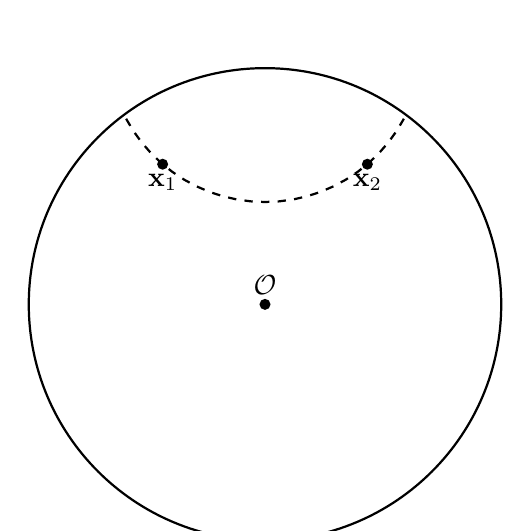
\begin{tikzpicture}
    % Draw the unit circle (Poincaré disk boundary)
    \draw[thick] (0,0) circle (3);
    % Draw the geodesic arc
    \draw[dashed, thick] plot[domain=-1.08:1.08] ({2*sin(\x r)},{-2*cos(\x r) + 3.3});
    % Draw points
    \fill (0,0) circle (0.07) node[above] {$\mathcal O$};
    \fill (-1.3,1.78) circle (0.07) node[below] {$\mathbf x_1$};
    \fill (1.3,1.78) circle (0.07) node[below] {$\mathbf x_2$};
  \end{tikzpicture}
  \caption{Poincaré disk with a geodesic between two points.}
  \label{fig:poincare-disk}
\end{figure}

\subsection{Hierarchical Clustering}

% TODO talk about the various clustering schemes mentioned in \cite{müllner2011modernhierarchicalagglomerativeclustering}, Figure 2. Mention how agglomerative clustering produces a tree, and how branch lengths in the tree are computed.

\subsection{Large Language Models and tokenizers}

Large language models (LLMs) are trained on vast amounts of internet text to learn the distribution over candidate tokens given a sequence of input tokens. An LLM's vocabulary is a set of tokens; each token is a string of characters. A common pre-processing step is to convert input text into a sequence of tokens via a \emph{tokenizer}.

Ultimately, an LLM ``sees'' tokens, so the choice of vocabulary crucial. One common way to choose tokens is to consider a sample body of text and choose the top $V$ most frequently occurring $n$-grams (over all $n\ge 1$). This results in many tokens being parts of words, which can be useful for capturing the structure of natural language.

% TODO cite something for transformer architecture
Most LLMs today use the transformer architecture, which uses self-attention mechanisms to model dependencies between tokens. First, the model learns token embeddings. In addition, the model learns projection matrices that map tokens into a latent space that better captures similarity structures. Each layer of the transformer uses this mechanism to allow tokens to ``pay attention'' to other tokens. As the input is passed through the layers, the model refines the meaning of each token in the context of the entire input.

After being trained on the internet, the model learns an internal representation of language that allows it to best complete input text. Ultimately, the distribution of candidate tokens output by an LLM is a function of the final hidden state of the model (i.e., the refined token embeddings at the last layer). Therefore, this final hidden state contains an abstract representation of the input text---suitable for downstream NLP tasks.

\subsection{Multi-Layer Perceptrons}

Multi-layer perceptrons (MLPs) are universal function approximators that work by feeding input data through an alternating series of linear and non-linear transformations. Namely, an MLP is a function $f: \mathbb{R}^i \rightarrow \mathbb{R}^o$ that maps data from an $i$-dimensional input space to an $o$-dimensional output space. Gradient descent is commonly used to train MLPs.

\section{Methodology}

We propose a novel method that takes as input an arbitrary set of computer files and organizes them into a nested tree of directories. Examples repositories containing files in a hierarchical directory structure is used to train a ``generative'' model that can then organize unseen files.

  [Illustration of input (flat files) to output (file tree)]

Such a model can be trained on different example repositories to produce models that perform well in different contexts. For example, training on GitHub repositories will produce a model that organizes files in a way that is useful for software projects. Meanwhile, training on, say, the filesystem of an operating system will produce a model that is better adapted to organizing non-text (binary) files. The latter case may be particularly useful for, say, organizing a user's internet downloads.

  % TODO: move above description/motivation to introduction???

  [Flow chart of the three parts]

Our method consists of three parts:

\begin{enumerate}
  \item Map files to feature vectors with the help of a pre-trained LLM. Namely, given a file $u_i$, the feature vector $x_i = \phi(u_i)$ should capture useful semantic information about the file. There are no learned parameters in this part.
  \item Learn a function $f$ that embeds file feature vectors into a low-dimensional metric space $(Y, \sigma)$. The mapping should preserve the true tree distance between files. We experiment with Euclidean and hyperbolic target spaces. Fuerthermore, we take $f$ to be an MLP.
  \item Organize a given set of files $\qty{u_1, u_2, \dots}$ hierarchically, with the end goal of creating a directory tree containing the files (physically, on disk). New/unseen files are feature expanded via $\phi$ and embedded into $(Y, \sigma)$ using the learned function $f$. Hierarchical clustering is then performed on the embedded files to create the directory tree.
\end{enumerate}

\subsection{Summary of Notation}

Below is a summary of the notation that is used throughout the rest of the report:

\begin{itemize}
  \item $u_i \in U$: a file from the space of all files.
  \item $U_\text{train}, U_\text{test} \subset U$: the set of training and test files, respectively.
  \item $\mathcal T(u_i, u_j)$: the true file tree distance between training files $u_i, u_j \in U_\text{train}$. Note that $(U_\text{train}, \mathcal T)$ forms a metric space.
  \item $x_i \in X = \mathbb{R}^d$: the feature vector of file $u_i$.
  \item $\phi: U \to X$: a fixed function that maps files to feature vectors.
  \item $f: X \to Y$: a learned function that embeds file feature vectors into a metric space, preserving distances.
  \item $(Y, \sigma)$: the target metric space in which we perform hierarchical clustering of files. For Euclidean spaces, we write $Y = \mathbb R^D$. For hyperbolic spaces, we write $Y = \mathcal H^D$.
  \item $d$: the dimensionality of the feature vectors.
  \item $D$: the dimensionality of the target metric space.
  \item $\Sigma^*$: the set of all strings, formed from a standard alphabet $\Sigma$.
\end{itemize}

\subsection{Part 1: Mapping Files to Feature Vectors}

Let $U$ be the space of all files. We start by defining a fixed, deterministic mapping $\phi: U \to X$ that maps files into $d$-dimensional feature vectors ($X = \mathbb R^d$). These file features should be suitable for downstream file embedding and clustering tasks. Specifically, for a given file, we are interested in properties that correlate with its location in the file system tree.

For notation, let $\Sigma$ be the set of characters in a standard alphabet, e.g., ASCII ($\abs{\Sigma} = 128$), or more generally, Unicode. Let $\Sigma^*$ denote the infinite set of all character strings. In our case, we look at a file's name and contents, ignoring other metadata like creation date and owner.

Given a file $u_i \in U$, we denote these properties as $\textsc{Filename}_i \in \Sigma^*$ and $\textsc{Contents}_i \in \Sigma^*$. (We will deal with non-text files later.) Ultimately, then, we care about a \emph{string-to-feature} function $f_s: \Sigma^* \to \mathbb R^{d/2}$, such that the overall file feature vector is the following concatenation:
\begin{align}
  \phi(u_i) =
  \Big( f_s(\textsc{Filename}_i), f_s(\textsc{Contents}_i) \Big) \in \mathbb R^d \; .
\end{align}

We propose two constructions of $f_s$, the string-to-feature function.

\subsubsection{String-to-Feature Construction 1: Counts of Top Tokens}

Do token counts capture enough semantic meaning to be useful for predicting file system tree distances?

Let $s \in \Sigma^*$ be the input string to $f_s$. Furthermore, we consider the top $t$ tokens of the pre-trained LLM's tokenizer.\footnote{Roughly speaking, these tokens are the $t$ most frequently seen $n$-grams during the LLM's training. Given no other \emph{a priori} information about file contents, we believe relying on a pre-trained tokenizer (which has been fitted on vast sums of internet text) is a reasonable way to discretize input strings.} We then compute
\begin{align}
  f_s(s) = \Big( \text{count}_1(s), \text{count}_2(s), \dots, \text{count}_t(s) \Big) \; ,
\end{align}
where $\text{count}_i(s)$ is the number of times the $i$-th most frequent token appears in the tokenized version of $s$. This construction yields $d = 2t$.

\subsubsection{String-to-Feature Construction 2: Last Hidden State of LLM}

We can also use the last hidden state of the LLM as the feature vector. This is a common practice in NLP, as the last hidden state is thought to contain a compressed representation of the input text. Namely, our LLMs have been pre-trained over vast sums of text such that the last hidden state represents the input text in a way that is useful for next-token prediction.

In general, if $d_k$ is the token embedding dimension of the LLM, and $\abs{s}$ is the number of tokens in $s$, then the last hidden state is a $\mathbb R^{\abs{s} \times d_k}$ matrix. It contains the \emph{refined} $d_k$-dimensional embedding of each input token. To produce the final feature vector, it is common practice to either average the token embeddings across the $\abs{s}$ tokens or take the embedding of the last token. The idea behind the latter strategy is that by the time the input has passed through the various self-attention layers, the last token's embedding has been adjusted to incorporate information from preceding tokens.

Furthermore, when using the last token embedding, we can employ the the \emph{Explicit One word Limitation (PromptEOL)} strategy described in \cite{jiang2023scalingsentenceembeddingslarge}, where we wrap the input \texttt{string} in the template:
\begin{center}
  \texttt{This file content: " [string] " contains in one word: "}
\end{center}
This strategy has been shown to improve the relevance of the last token embedding.

\textbf{A potential worry} is that the distribution of \textsc{Filename} and \textsc{Contents} strings are, in general, quite different from the natural language text that LLMs are trained on. Still, we believe that tokenization and subsequent embedding captures interesting details. For \textsc{Filename}, we may want to identify strings like \texttt{foo-test.js} and \texttt{bar-test.js}, which correspond files in the same \texttt{src/\_\_tests\_\_} directory. Both names may contain the shared tokens \texttt{["test", ".js"]}, so passing the names through the LLM should produce similar hidden state embeddings. Similarly, for \textsc{Contents}, HTML files may contain many \texttt{<div>} tokens, and these tokens should have similar influences on the hidden state.

At minimum, the hidden state can be seen as capturing info similar to the token counts in the previous construction.

\subsection{Part 2: Learning the Embedding Function}

This part learns a distance-preserving embedding function $f: X \to Y$ that embeds the feature vectors into a low-dimensional metric space $(Y, \sigma)$. For the learning process, we consider using training files $U_\text{train} \subset U$ that exist in a known file system tree (e.g., files from a GitHub repository). For these training files, the true tree distance $\mathcal T(u_i, u_j)$ is known for all $u_i, u_j \in U_\text{train}$. Therefore, the training files existing in a metric space $(U_\text{train}, \mathcal T)$. Of course, for each file, we first compute $x_i = \phi(u_i) \in X$.

We take $f$ to be a multi-layer perceptron (MLP). The goal is to learn a mapping that minimizes the discrepancy between true tree distances $\mathcal T$ and distances $\sigma$ in the target metric space. We study two different cost functions that quantify this discrepancy.

\subsubsection{Cost Function 1: Mean Squared Error}

The obvious strategy is to minimize the mean squared error of distances between all $\abs{U}^2$ pairs of files. Namely, with $\mathbf w$ denoting the parameters of $f$, and $x_i = \phi(u_i)$, we optimize the following:
\begin{align*}
  \min_{\mathbf w} \sum_{(u_i, u_j) \in U^2} \Big[ \sigma(f(x_i), f(x_j)) - \mathcal T(u_i, u_j) \Big]^2 \; .
\end{align*}

\subsubsection{Cost Function 2: t-SNE Objective}

% TODO

\subsubsection{Normalizing MLP Output into the Poincaré Disk (or Ball)}

Recall that an MLP outputs vectors in $\mathbb R^D$. This is fine for Euclidean spaces ($Y = \mathbb R^D$). However, for hyperbolic spaces, we use the Poincaré disk model, which requires the output to be in $\mathcal H^D$. Namely, the output must be in the unit ball $\qty{\mathbf y \in \mathbb R^D : \norm{\mathbf y} < 1}$. This requires us to use some normalization technique.

The simplest strategy is to clip the output norms to $1-\epsilon$, where $\epsilon$ is sufficiently large to avoid numeric issues that arise when computing distances near the edge of the Poincaré disk. This strategy is problematic in practice because embedded points get ``stuck'' at the boundary of the disk, due to embedding gradients being zero in the radial direction after clipping.

\begin{figure}[ht]
  \centering
  \begin{tikzpicture}
    % Draw the unit circle (Poincaré disk boundary)
    \draw[thick] (0,0) circle (3);
    % Draw the smaller dotted circle (1 - epsilon)
    \draw[thick, dotted] (0,0) circle (2.7);
    % Draw radial lines from the origin to the points (going past the boundary)
    \draw[dotted] (0,0) -- (4, 0);
    \draw[dotted] (0,0) -- (-4, 0);
    \draw[dotted] (0,0) -- (0, 4);
    \draw[dotted] (0,0) -- (0, -4);
    \draw[dotted] (0,0) -- (2.83, 2.83);
    \draw[dotted] (0,0) -- (-2.83, -2.83);
    % Place points on the smaller circle
    \fill (2.7, 0) circle (0.05);
    \fill (-2.7, 0) circle (0.05);
    \fill (0, 2.7) circle (0.05);
    \fill (0, -2.7) circle (0.05);
    \fill (1.91, 1.91) circle (0.05);
    \fill (-1.91, -1.91) circle (0.05);
    % Draw original points outside the disk (fill + outline)
    \fill[white] (3.5, 0) circle (0.05);
    \draw[gray]  (3.5, 0) circle (0.05);
    \fill[white] (-3.3, 0) circle (0.05);
    \draw[gray]  (-3.3, 0) circle (0.05);
    \fill[white] (0, 3.8) circle (0.05);
    \draw[gray]  (0, 3.8) circle (0.05);
    \fill[white] (0, -3.7) circle (0.05);
    \draw[gray]  (0, -3.7) circle (0.05);
    \fill[white] (2.5, 2.5) circle (0.05);
    \draw[gray]  (2.5, 2.5) circle (0.05);
    \fill[white] (-2.7, -2.7) circle (0.05);
    \draw[gray]  (-2.7, -2.7) circle (0.05);
  \end{tikzpicture}
  \caption{Poincaré disk with embedded points clipped to radius $1 - \epsilon$.}
  \label{fig:poincare-disk-epsilon}
\end{figure}

Ideally, we want points to get arbitrarily close to the boundary of the Poincaré disk. This is because there is more \emph{space} to fit tree-like structures near the boundary. Furthermore, we want a strategy that reserves ``more bits'' of floating point precision for regions near the boundary. One such strategy is to use apply a nonlinear transformation $g: \mathbb R^+ \to [0, 1)$ to the norms of MLP-outputted vectors. $g(r) = \tanh(r)$ is a possible candidate, as $\dv{g}{r}$ diminishes for small $r$. In other words, a large share of the domain $r \in \mathbb R^+$ is mapped to the region near $1$ in $[0, 1)$.

We instead choose to use a very similar transformation:
\begin{align}
  g(r) = \sqrt{1 - e^{-r^2}} \; . \label{eq:radial-transformation}
\end{align}

\begin{figure}[ht]
  \centering
  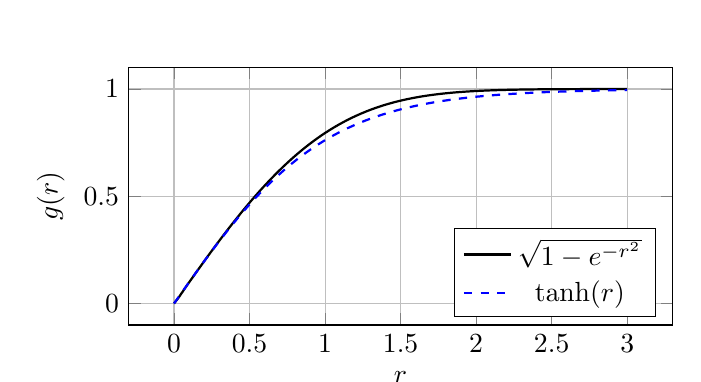
\begin{tikzpicture}
    \begin{axis}[
        xlabel={$r$},
        ylabel={$g(r)$},
        legend pos=south east,
        grid=both,
        width=0.7\textwidth,
        height=0.4\textwidth,
      ]
      \addplot[
        domain=0:3,
        samples=100,
        black,
        thick,
      ] {sqrt(1 - exp(-x^2))};
      \addlegendentry{$\sqrt{1 - e^{-r^2}}$}
      \addplot[
        domain=0:3,
        samples=100,
        blue,
        dashed,
        thick,
      ] {tanh(x)};
      \addlegendentry{$\tanh(r)$}
    \end{axis}
  \end{tikzpicture}
  \caption{Comparison of $g(r) = \tanh(r)$ and $g(r) = \sqrt{1 - e^{-r^2}}$.}
  \label{fig:radial-transformations}
\end{figure}

This particular formulation has the advantage of simplifying the Poincaré distance expression in \eqref{eq:poincare-distance}. Namely, let $y_i = f(x_i)$ be the output of the MLP, and consider computing the Poincaré distance between output vectors \emph{normalized} via $g$.\footnote{Abusing notation, we will let $g(y_i)$ denote a \emph{vector} that is in the direction of $y_i$ but with norm equal to $g(\norm{y_i})$.} The quantity in the denominator simplifies through $1 - \norm{g(y_i)}^2 = e^{-\norm{y_i}^2}$. The Poincaré metric---accounting for normalization---is then\footnote{In practice, we must also add a small $10^{-7}$ epsilon to the argument of $\text{arcosh}(\cdot)$ to avoid numerical issues.}
\begin{align}
  \sigma(y_i, y_j)
  = d \Big( g(y_i), g(y_j) \Big)
  = \text{arcosh} \qty[1 + 2 \frac{\norm{g(y_i) - g(y_j)}^2}{e^{-\norm{y_i}^2} e^{-\norm{y_j}^2}}] \; .
\end{align}

\begin{figure}[ht]
  \centering
  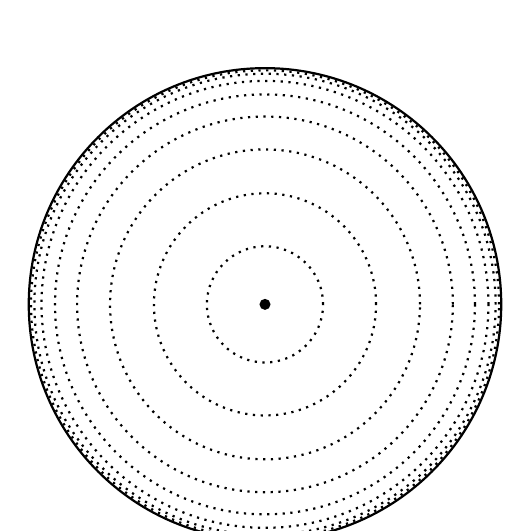
\begin{tikzpicture}
    % Draw the unit circle (Poincaré disk boundary)
    \draw[thick] (0,0) circle (3);
    % Draw level curves at every 0.25 (pre-transformed)
    \draw[thick, dotted] (0,0) circle (0.738);
    \draw[thick, dotted] (0,0) circle (1.411);
    \draw[thick, dotted] (0,0) circle (1.968);
    \draw[thick, dotted] (0,0) circle (2.386);
    \draw[thick, dotted] (0,0) circle (2.667);
    \draw[thick, dotted] (0,0) circle (2.838);
    \draw[thick, dotted] (0,0) circle (2.929);
    \draw[thick, dotted] (0,0) circle (2.972);
    % Draw the origin
    \fill (0,0) circle (0.07);
  \end{tikzpicture}
  \caption{Level curves in the Poincaré disk at normalized radii $g(0.25), g(0.5), \dots, g(2.0)$. Observe that more ``input bits'' are reserved for the boundary of the disk.}
  \label{fig:poincare-level-curves}
\end{figure}


\subsection{Part 3: Organizing Files Hierarchically}

Finally, we propose a procedure to organize files hierarchically. Here, we consider ``test'' files $U_\text{test} \subset U$ whose true tree distances are unknown. These files have not been used to train the embedding function $f$.

Using the fixed feature expansion and learned embedding function, we can embed each test file into the target space $(Y, \sigma)$. Namely, we compute $y_i = f(\phi(u_i))$ for all $u_i \in U_\text{test}$.

Then, we utilize standard agglomerative hierarchical clustering methods to organize the embedded files into a tree. Our method supports the various clustering schemes listed in \cite{müllner2011modernhierarchicalagglomerativeclustering}, including \texttt{single}, \texttt{complete}, and \texttt{Ward}. We use \texttt{scipy.cluster.hierarchy.linkage} from SciPy to perform the clustering. The resulting tree is used to produce a directory structure in which the files are then placed.

The user specifies a \texttt{num\_dirs} parameter (e.g., 10) that specifies exactly how many directories are to appear in the final directory hierarchy. The top \texttt{num\_dirs} longest edges in the cluster tree are ``cut''; at each cut, a new directory is created to contain the subtree.

\begin{figure}[ht]
  \centering
  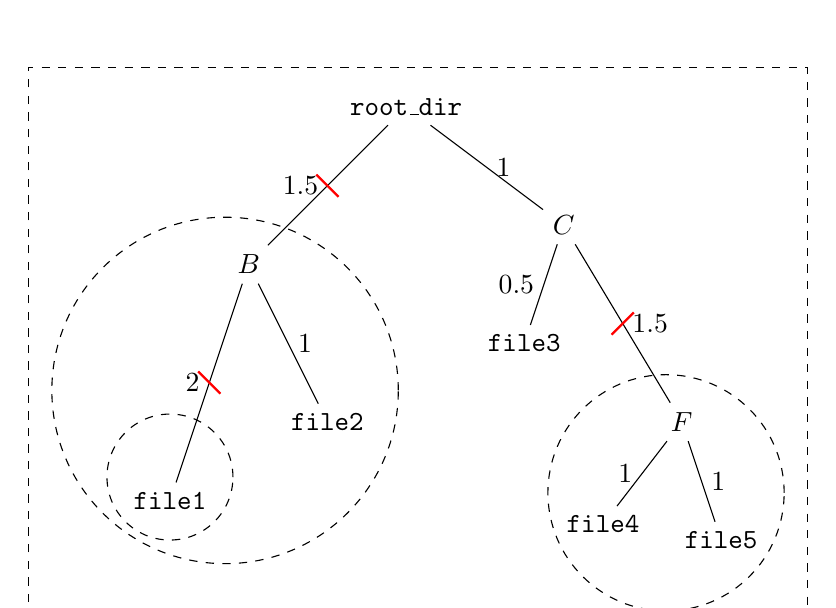
\begin{tikzpicture}
    % Define nodes
    \node (A) at (0,0) {\texttt{root\_dir}};
    \node (B) at (-2,-2) {$B$};
    \node (C) at (2,-1.5) {$C$};
    \node (D) at (-3,-5) {\texttt{file1}};
    \node (E) at (-1,-4) {\texttt{file2}};
    \node (F) at (3.5,-4) {$F$};
    \node (G) at (1.5,-3) {\texttt{file3}};
    \node (H) at (2.5,-5.3) {\texttt{file4}};
    \node (I) at (4,-5.5) {\texttt{file5}};

    % Draw edges with varying lengths
    \draw (A) -- node[midway, left] {$1.5$} (B);
    \draw (A) -- node[midway, right] {$1$} (C);
    \draw (B) -- node[midway, left] {$2$} (D);
    \draw (B) -- node[midway, right] {$1$} (E);
    \draw (C) -- node[midway, right] {$1.5$} (F);
    \draw (C) -- node[midway, left] {$0.5$} (G);
    \draw (F) -- node[midway, left] {$1$} (H);
    \draw (F) -- node[midway, right] {$1$} (I);

    % Cut the top 3 longest edges
    % Edges: (A)-(B), (B)-(D), (C)-(F)
    \draw[red, thick] ($(A)!0.5!(B)$) -- ++(135:0.2) -- ++(-45:0.4);
    \draw[red, thick] ($(B)!0.5!(D)$) -- ++(135:0.2) -- ++(-45:0.4);
    \draw[red, thick] ($(C)!0.5!(F)$) -- ++(45:0.2) -- ++(-135:0.4);

    % Draw circles around subtrees in new directories
    \draw[dashed] (-2.3,-3.6) circle (2.2);
    \draw[dashed] (-3.0,-4.7) circle (0.8);
    \draw[dashed] (3.3,-4.9) circle (1.5);

    % Surround whole tree in a rectangle
    \draw[dashed] (-4.8,-6.5) rectangle (5.1,0.5);

  \end{tikzpicture}
  \caption{A tree with varying branch lengths. The top \texttt{num\_dirs=3} longest edges are cut to create new directories (shown in dashed lines).}
  \label{fig:example-tree-with-cuts}
\end{figure}

\begin{figure}[ht]
  \centering
  \begin{BVerbatim}
    root_dir
    ├── dir1
    │   ├── dir2
    │   │   └── file1
    │   └── file2
    ├── dir3
    │   ├── file4
    │   └── file5
    └── file3
  \end{BVerbatim}
  \caption{The directory structure produced from the tree in Figure \ref{fig:example-tree-with-cuts}.}
  \label{fig:example-directory-structure}
\end{figure}

\subsection{Time Complexity Analysis}

\section{Experiments}

\section{Conclusion}


\printbibliography

\end{document}
